%% ============================================================
%% methods.tex  —  Chapter 2
%% ============================================================
\chapter{Methods}
\label{ch:methods}

Note: Acronyms and notation are defined in Appendix \ref{app:notation}

\section{Overview of the Analytical Approach}
\label{sec:overview}

The framework proceeds in the following stages:
\begin{enumerate}
    \item A one-off data-acquisition stage to gather relevant datasets from varied raw and derived sources. Details are presented in Appendix \ref{app:data_sources}
    \item A data preprocessing stage: e.g. some map data needs converting into a canonical mapping projection so that different features can be computed/extracted from the same Titan location. The canonical format used is 
        \begin{enumerate}
            \item Projection: SimpleCylindrical (equirectangular) 
            \item Titan sphere: R=2,575,000 m
            \item Longitude: West-positive, 0\textdegree~\rightarrow~360\textdegree,    (matches all USGS raster products)
            \item Latitude: North-up, +90\textdegree~\rightarrow~-90\textdegree
        \end{enumerate}
    \item Extraction of 8 habitability-proxy features from the data, details in sections \ref{sec:data}, \ref{sec:features}.
    \item Bayesian conjugate updating to produce a posterior habitability probability map at each of five named geological 'anchor' epochs, (\textit{Past}, \textit{Lake Formation}, \textit{Present}, \textit{Near Future}, \textit{Future}). Details are presented in \ref{sec:bayes}
    % \item Temporal scaling of features between anchor epochs to produce 72 geological epochs from $-3.8\gya$ to $+6.5\gya$ 
    \item Outputs: Graphs and ranking of named surface sites by posterior probability for each epoch. Details in \ref{sec:temporal_configs}
\end{enumerate}

Figure~\ref{fig:pipeline} provides a schematic overview of the five-stage
analytical pipeline from data acquisition to visualisation.

\begin{figure}[H]
  \centering
  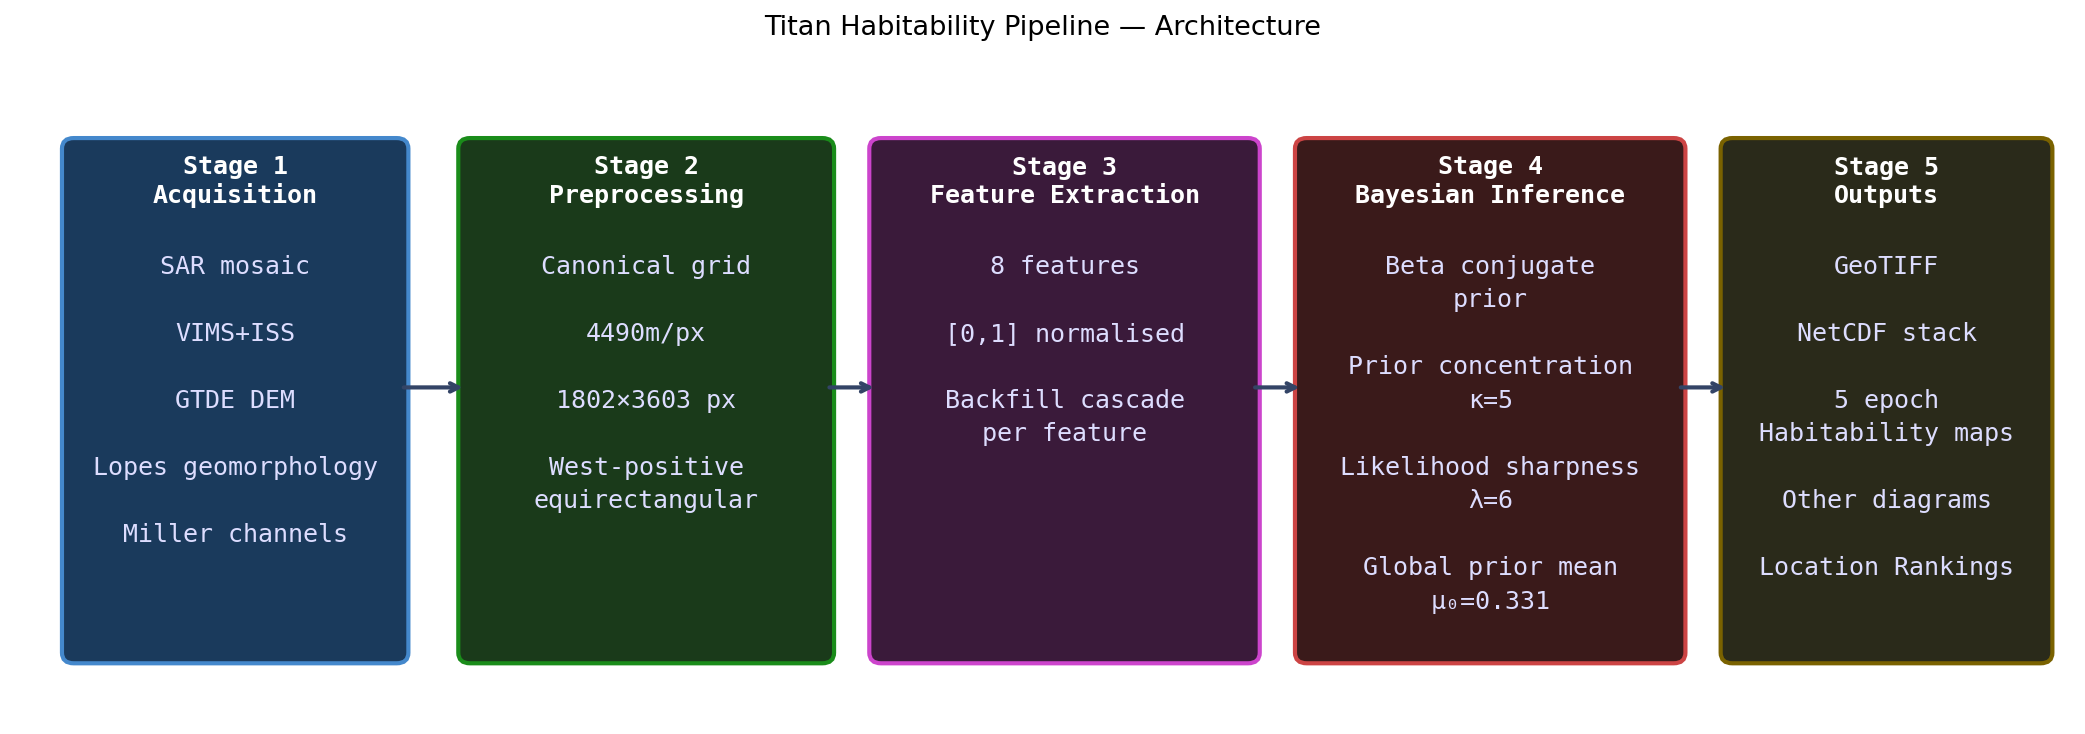
\includegraphics[width=\textwidth]{images/pipeline_flowchart.png}
  \caption{Schematic overview of the five-stage Titan habitability analysis
    pipeline.  All eight habitability-proxy features are extracted in Stage 3
    and combined in the Bayesian posterior update of Stage 4 to produce
    $P(H \mid \featurevec)$ maps at each of the five epochs.}
  \label{fig:pipeline}
\end{figure}

The Bayesian approach taken in this thesis requires explanation and follows next.

\subsection{The Bayesian Approach: Motivation and Structure}
\label{sec:bayes_intro}

The central methodological challenge in quantifying \titan{}'s surface
habitability is that no single Cassini instrument directly measures
habitability.  Each instrument provides a partial and indirect proxy: radar
backscatter reveals surface composition and liquid surfaces; near-infrared
spectroscopy constrains organic content; thermal emission maps the temperature
field that drives the methane cycle; altimetry constrains topography and hence
organic accumulation patterns; and the geomorphological classification
synthesises the collective information from all instruments into terrain types
whose habitability implications can be grounded in laboratory and theoretical
work.

The approach taken here is to combine these partial proxies through a Bayesian
inference framework that produces, at each grid cell, a posterior probability
of habitability $P(H \mid \featurevec)$ given the vector of observed features
$\featurevec = (f_1, \ldots, f_8)$.  This is structurally analogous to the
approach of \citet{Affholder2021}, who used Bayesian methods to evaluate
whether the observed methane flux in Enceladus's plumes is more consistent
with abiotic serpentinisation or with biological methanogenesis.  The key
extensions here are spatial resolution (a 6.49-million-pixel global map rather
than a single-point estimate), the number of independent observational inputs
(eight features rather than one), and the temporal scope (five epochs spanning
geological time rather than a single snapshot).

The structure of the inference is: 
\begin{enumerate}
    \item encode prior knowledge about
\titan{}'s habitability into a probability distribution over the latent
variable $H$;
    \item update that distribution using each observed feature
$f_i$ as evidence;
    \item report the resulting posterior probability
$P(H \mid \featurevec)$ as the habitability estimate at each pixel.
\end{enumerate}

The Bayesian inference and subsequernt analysis is applied at \SI{4490}{\metre\per\text{px}} resolution on a
canonical equirectangular grid covering the full globe (1802 pixels in
latitude $\times$ 3603 pixels in longitude), using a west-positive longitude
convention consistent with all Cassini raster products.  This resolution is
chosen to match the coarsest primary dataset (the GTDR altimetry mosaic at
$\sim$22\,km per pixel) whilst resolving lake margins and fluvial features
at $\sim$45\,km scale.  All eight input datasets are reprojected to this
common grid before feature extraction.


\section{Observational Data Sources}
\label{sec:data}

Eight Cassini data products are used, summarised in Table~\ref{tab:data_sources}.  Processing details are in Appendix~\ref{app:notation}.

\begin{table}[H]
\centering
\small
\caption{Cassini data sources used in the habitability framework.}
\label{tab:data_sources}
\begin{tabular}{p{5.2cm}p{2.6cm}p{5.8cm}}
\toprule
\textbf{Dataset} & \textbf{Coverage} & \textbf{Habitability feature} \\
\midrule
Cassini SAR mosaic      & $\sim$67\% surface & $f_1$ liquid hydrocarbon; $f_7$ geodiversity \\
VIMS 1.59/1.27\,\textmu{}m & $\sim$50\% surface & $f_2$ organic abundance \\
CIRS thermal mosaic     & Global ($\sim$10\textdegree{}) & $f_4$ methane cycle; $f_5$ surf--atm \\
GTDE/GTDR DEM           & $\sim$90\% (interp.) & $f_6$ topographic complexity \\
Lopes (2019) geomorphology\ map & $\sim$90\% SAR & $f_2$ organic; $f_7$ geodiversity \\
Miller (2021) channel map   & SAR coverage     & $f_5$ surface--atmosphere \\
Hedgepeth (2020) craters & SAR coverage      & $f_7$ geodiversity; past epoch \\
Tidal $k_2$ (global)    & Global scalar      & $f_8$ subsurface ocean \\
\bottomrule
\end{tabular}
\end{table}

\section{Feature Extraction}
\label{sec:features}

Eight habitability-proxy features $f_1$--$f_8$ are extracted from the data sources above, each normalised to $[0,1]$ via robust percentile clipping (2nd--98th percentile; Eq.~\ref{eq:normalise}).  Table~\ref{tab:feature_summary} summarises the features, their prior weights, prior means, and scientific basis.  Full engineering details --- data processing, normalisation choices, seam-correction rationale for $f_2$, and backfill procedures --- are in Appendix~\ref{app:features}.

\begin{equation}
  \hat{f}_i = \mathrm{clip}\!\left(
    \frac{f_i - f_{i,\text{p2}}}{f_{i,\text{p98}} - f_{i,\text{p2}}},
    \; 0, \; 1
  \right)
  \label{eq:normalise}
\end{equation}

\begin{table}[H]
\centering
\small
\caption{The eight habitability-proxy features.  Weight $w_i$ and prior mean
  $\mu_i$ are the present-epoch values used in the Bayesian update
  (Eq.~\ref{eq:posterior_mean}).  $\mu_0 = \sum_i w_i\mu_i = 0.331$.}
\label{tab:feature_summary}
\begin{tabular}{clp{0.5cm}p{0.6cm}p{6.0cm}}
\toprule
\textbf{$f_i$} & \textbf{Name} & $w_i$ & $\mu_i$ & \textbf{Scientific rationale} \\
\midrule
$f_1$ & Liquid hydrocarbon availability  & 0.25 & 0.02  & Direct solvent for non-aqueous biochemistry \citep{McKaySmith2005} \\
$f_2$ & Organic abundance       & 0.20 & 0.70  & Tholin substrate for prebiotic chemistry \citep{MeyerDombard2025} \\
$f_3$ & Chemical energy (acetylene) & 0.20 & 0.35 & Acetylenotrophy energy proxy \citep{McKaySmith2005,Yanez2024} \\
$f_4$ & Methane cycle intensity & 0.15 & 0.40  & Solvent transport and chemical concentration cycling \\
$f_5$ & Surface--atm.\ interaction & 0.08 & 0.35 & Atmospheric delivery of organics and energy substrates \\
$f_6$ & Topographic complexity  & 0.06 & 0.25  & Microenvironment diversity and chemical gradient maintenance \\
$f_7$ & Geomorphological diversity & 0.04 & 0.30 & Terrain heterogeneity proxy for ecological niche richness \\
$f_8$ & Subsurface ocean proximity & 0.02 & 0.03 & Potential water-chemistry conduit; SAR-bright annuli \citep{Iess2012} \\
\bottomrule
\end{tabular}
\end{table}

Figure~\ref{fig:feature_panel} shows all eight feature maps at the present epoch; Figure~\ref{fig:epoch_timeline} shows how each feature is modulated across geological time.

\section{Bayesian Inference Model}
\label{sec:bayes}

\subsection{Formulation: Latent Variables, Conjugacy, and the Beta-Binomial Model}
\label{sec:bayes_motivation}

\paragraph{The latent variable.}
In this framework, habitability $H$ is treated as a \textit{latent variable}
--- a quantity that cannot be directly observed by any Cassini instrument but
whose value is inferred from the combination of observational proxies
$\featurevec = (f_1, \ldots, f_8)$.  A latent variable (from the Latin
\textit{latere}: to be hidden) influences observable outcomes but is not
itself directly measurable.  Here, $H$ is not a binary yes-or-no property
but a continuous probability in $[0, 1]$: the value $H = p$ at a given pixel
means that pixel has probability $p$ of satisfying the relevant habitability
conditions given all available evidence.  Each feature $f_i$ provides partial,
indirect evidence about the value of $H$.

\paragraph{Why a Beta distribution?}
The Beta distribution $\mathrm{Beta}(\alpha, \beta)$ is defined on $[0, 1]$
and characterised by two positive shape parameters $\alpha$ and $\beta$.
It is unimodal when both $\alpha > 1$ and $\beta > 1$, with mean
$\alpha/(\alpha + \beta)$ and variance that decreases as $\alpha + \beta$
grows.  Because it is bounded on $[0,1]$ and can represent any unimodal
belief over a probability, it is the natural prior for the latent
habitability probability $H$.

\paragraph{Conjugacy explained.}
A prior distribution is \textit{conjugate} to a likelihood function if the
posterior (prior updated by data) has the same mathematical form as the
prior, differing only in its parameter values.  The Beta distribution is
conjugate to the Binomial likelihood: if the prior on a success probability
$p$ is $\mathrm{Beta}(\alpha_0, \beta_0)$ and we observe $k$ successes
in $n$ Bernoulli trials, the posterior is
$\mathrm{Beta}(\alpha_0 + k,\; \beta_0 + (n - k))$.
This analytical tractability makes the update feasible at 6.49 million
pixels simultaneously with no numerical integration required.

\paragraph{The Beta-Binomial model.}
Each feature $f_i \in [0, 1]$ is treated as the fractional outcome of
$\lambda w_i$ virtual Bernoulli trials: fraction $f_i$ of those trials are
``successes'' (evidence for habitability) and $(1 - f_i)$ are ``failures''
(evidence against).  High feature values contribute more positive
pseudo-observations and shift the posterior towards higher habitability;
low values do the opposite.  The prior contributes $\kappa$ virtual
observations and the data from all eight features contribute a further
$\lambda \sum_i w_i = \lambda$ observations.
Figure~\ref{fig:beta_update} visualises the updating process for three
representative sites (Kraken southern shore, Belet dune field, Selk crater),
showing how each successive feature narrows and displaces the Beta
distribution from the prior to the final posterior.  The figure also
shows the 95\%~HDI for eight key present-epoch sites.

Figure~\ref{fig:bayes_update} illustrates this update graphically for four
representative sites.  The left panel shows the prior
$\mathrm{Beta}(\alpha_0, \beta_0)$, which is weakly informative
($\sigma \approx 0.18$) and centred at $\mu_0 = 0.331$.  The right panel
shows the posteriors after incorporating the respective Cassini feature
values: the Kraken Mare shoreline and Ligeia shoreline shift rightward
(high liquid, methane-cycle, and geodiversity scores), while the Belet dune
sea shifts only modestly (high organic but no liquid) and Selk crater shifts
leftward (below-average methane cycle and surface--atmosphere scores despite
exceptional geodiversity).

\begin{figure}[H]
  \centering
  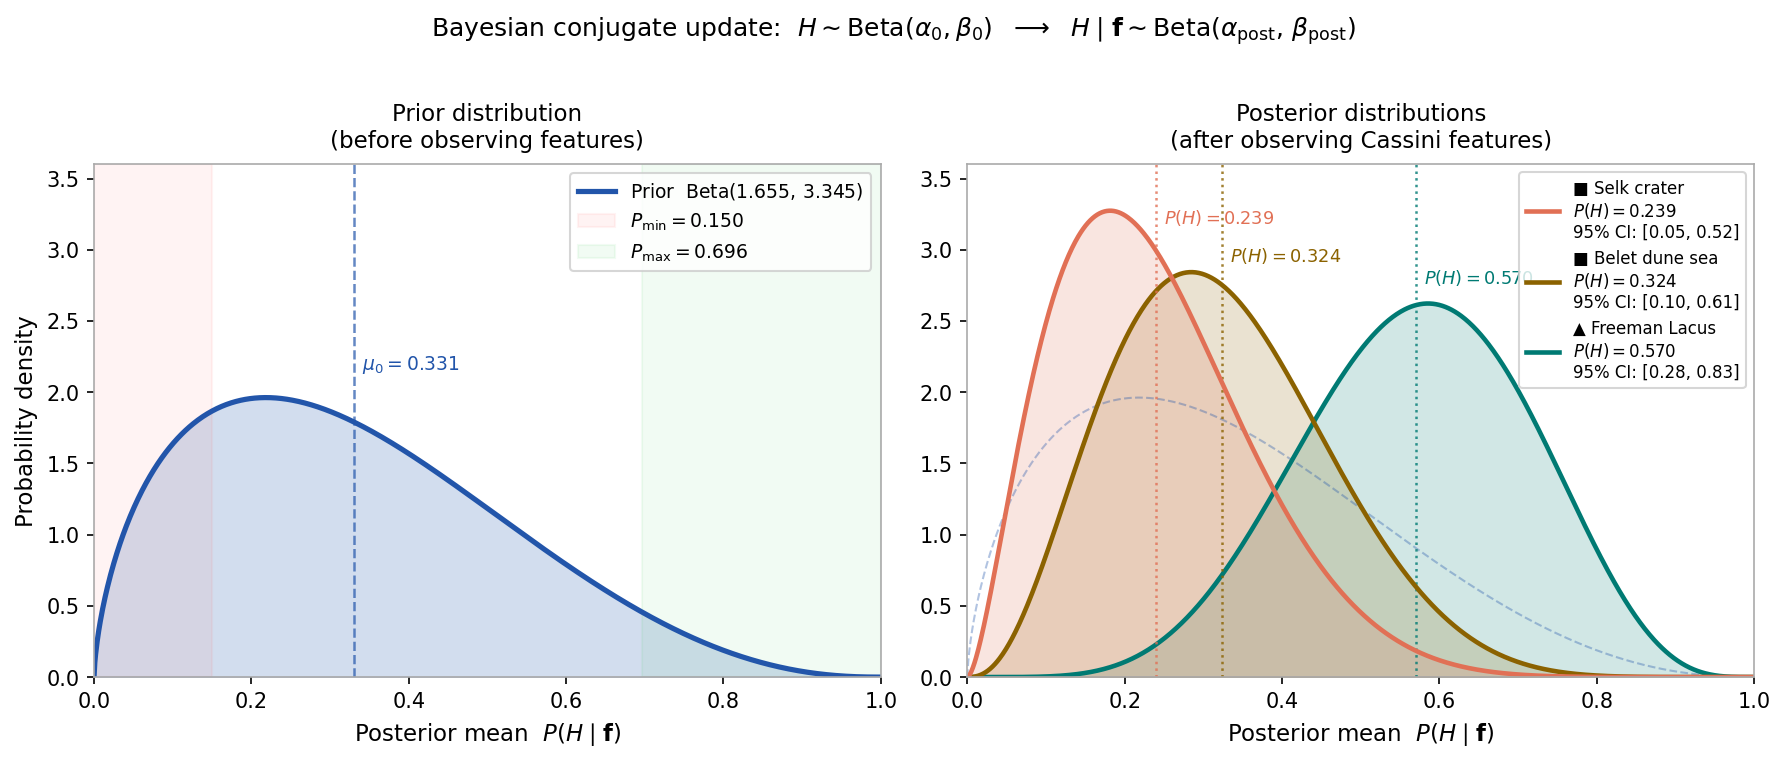
\includegraphics[width=\textwidth]{images/fig_bayesian_update.png}
  \caption{Beta-conjugate Bayesian update for four representative \titan{}
    surface environments.  \textit{Left:} the prior distribution
    $H \sim \mathrm{Beta}(1.655,\,3.345)$ with mean $\mu_0 = 0.331$.
    Shaded bands mark the hard bounds $[P_\text{min}, P_\text{max}] =
    [0.150, 0.696]$.  \textit{Right:} posterior distributions after
    incorporating the Cassini feature vector $\featurevec$ for each site
    (parameters $\kappa = 5$, $\lambda = 6$; present epoch).  The update
    sharpens and shifts each distribution in proportion to how far the
    site's weighted feature sum $\sum_i w_i f_i$ departs from the prior
    mean.  Polar lake shores (dark cyan/teal) shift markedly right; the equatorial
    crater (dark orange-red) shifts left; the dune sea (dark amber) remains near the prior.
    95\% HDI values are given in the legend.}
  \label{fig:bayes_update}
\end{figure}

\subsection{Prior Distribution}
\label{sec:prior}

The prior distribution over habitability at any pixel is:
\begin{equation}
  H \sim \mathrm{Beta}(\alpha_0, \beta_0), \qquad
  \alpha_0 = \mu_0\kappa, \quad \beta_0 = (1 - \mu_0)\kappa
  \label{eq:prior_dist}
\end{equation}
where $\mu_0$ is the global prior mean habitability and $\kappa$ is the
concentration parameter.  The parameter $\alpha_0$ counts prior
pseudo-successes (evidence for habitability) and $\beta_0$ counts prior
pseudo-failures.  The global prior mean is the weighted average of the
eight feature prior means:
\begin{equation}
  \mu_0 = \sum_{i=1}^{8} w_i \mu_i = 0.331
  \label{eq:prior_mean}
\end{equation}
This represents our best estimate that an average \titan{} pixel has
$\sim$33\% probability of habitability before examining the Cassini data.
The value reflects the combination of a large organic inventory
($w_2\mu_2 = 0.14$, the dominant term) tempered by limited liquid coverage
($w_1\mu_1 = 0.005$, the smallest term).  Full prior values are listed in
Appendix~\ref{app:priors}.

The concentration parameter $\kappa = 5$ controls how strongly the prior
resists updating: a larger $\kappa$ requires more data to shift the
posterior away from $\mu_0$.  The value $\kappa = 5$ was chosen to place
the prior and data on approximately equal footing ($\kappa/(\kappa+\lambda)
= 5/11 \approx 0.45$), reflecting the recognition that eight Cassini
observables provide genuine but imperfect information about habitability.
The likelihood sharpness $\lambda = 6$ similarly encodes the judgement that
a full set of ideal features ($f_i = 1$ for all $i$) should shift the
posterior from $\mu_0$ to $P_\text{max}$ but not to certainty.
A sensitivity analysis demonstrating robustness to variations of these
parameters is presented in Section~\ref{sec:sensitivity}.
With $\kappa = 5$:
\begin{equation}
  \alpha_0 = 0.331 \times 5 = 1.655, \qquad
  \beta_0 = 0.669 \times 5 = 3.345
\end{equation}
Both shape parameters exceed 1, ensuring a unimodal prior with interior
mode $\approx 0.17$ and standard deviation $\approx 0.18$ --- weakly
informative, encoding genuine pre-Cassini uncertainty.

\subsection{Posterior Update}
\label{sec:posterior_update}

Given observed features $\featurevec = (f_1, \ldots, f_8)$, the posterior
is obtained by Beta-Binomial conjugate updating:
\begin{equation}
  H \mid \featurevec \sim \mathrm{Beta}(\alpha_\text{post}, \beta_\text{post})
  \label{eq:posterior_dist}
\end{equation}
\begin{align}
  \alpha_\text{post}
    &= \underbrace{\alpha_0}_{\substack{\text{prior}\\\text{positives}}}
     + \underbrace{\lambda \sum_{i=1}^{8} w_i f_i}_{\substack{\text{data}\\\text{positives}}}
  \label{eq:alpha_post} \\[8pt]
  \beta_\text{post}
    &= \underbrace{\beta_0}_{\substack{\text{prior}\\\text{negatives}}}
     + \underbrace{\lambda \sum_{i=1}^{8} w_i (1 - f_i)}_{\substack{\text{data}\\\text{negatives}}}
  \label{eq:beta_post}
\end{align}

Each term has a transparent interpretation.
$\alpha_\text{post}$ accumulates all positive evidence: the prior
pseudo-successes $\alpha_0 = 1.655$ plus $\lambda w_i f_i$ data
pseudo-successes from each feature; it ranges from $\alpha_0$ (all $f_i = 0$)
to $\alpha_0 + \lambda = 7.655$ (all $f_i = 1$).
$\beta_\text{post}$ accumulates all negative evidence and varies reciprocally.
The total $\alpha_\text{post} + \beta_\text{post} = \kappa + \lambda = 11$
is constant for all pixels; only the split between positive and negative
evidence changes with the data.
The parameter $\lambda = 6.0$ is the \textit{likelihood sharpness parameter},
setting the total weight of the data relative to the prior weight $\kappa = 5$.

The posterior mean, the primary habitability score at each pixel, is:
\begin{equation}
  P(H \mid \featurevec)
  = \frac{\alpha_\text{post}}{\alpha_\text{post} + \beta_\text{post}}
  = \frac{1.655 + 6{\displaystyle\sum_i} w_i f_i}{11}
  \label{eq:posterior_mean}
\end{equation}
This is a convex combination of the prior mean $\mu_0$ (weight $5/11$) and
the data-driven score $\sum_i w_i f_i$ (weight $6/11$).  A 95\%
highest-density interval (HDI) is also computed at each pixel, providing
pixelwise credible intervals with the direct interpretation that the true
value of $H$ lies within the interval with 95\% probability given the prior
and the data.  The 95\% level is chosen for compatibility with conventional
confidence interval standards, facilitating direct comparison with
frequentist results in the literature; the practical difference from a
94\% or 89\% interval is negligible for the Beta distributions used here.

\subsection{Posterior Bounds}
\label{sec:bounds}

Since $\alpha_\text{post} + \beta_\text{post} = 11$ is constant, the
posterior mean satisfies hard limits:
\begin{equation}
  P_\text{min} = \frac{\alpha_0}{11} = \frac{1.655}{11} \approx 0.150,
  \qquad
  P_\text{max} = \frac{\alpha_0 + \lambda}{11} = \frac{7.655}{11} \approx 0.696
  \label{eq:bounds}
\end{equation}
These bounds exist because the prior contributes irreducible positive
($\alpha_0$) and negative ($\beta_0$) pseudo-observations that the data
cannot fully cancel.  Even a pixel with all eight features at maximum
($f_i = 1$ for all $i$) achieves only $P_\text{max} \approx 0.696$, not 1.0.
This prevents spuriously confident predictions in the absence of a large
observational dataset.  The colourbar for all maps is calibrated to
$[0.10, 0.75]$, spanning the achievable range.

\begin{figure}[H]
  \centering
  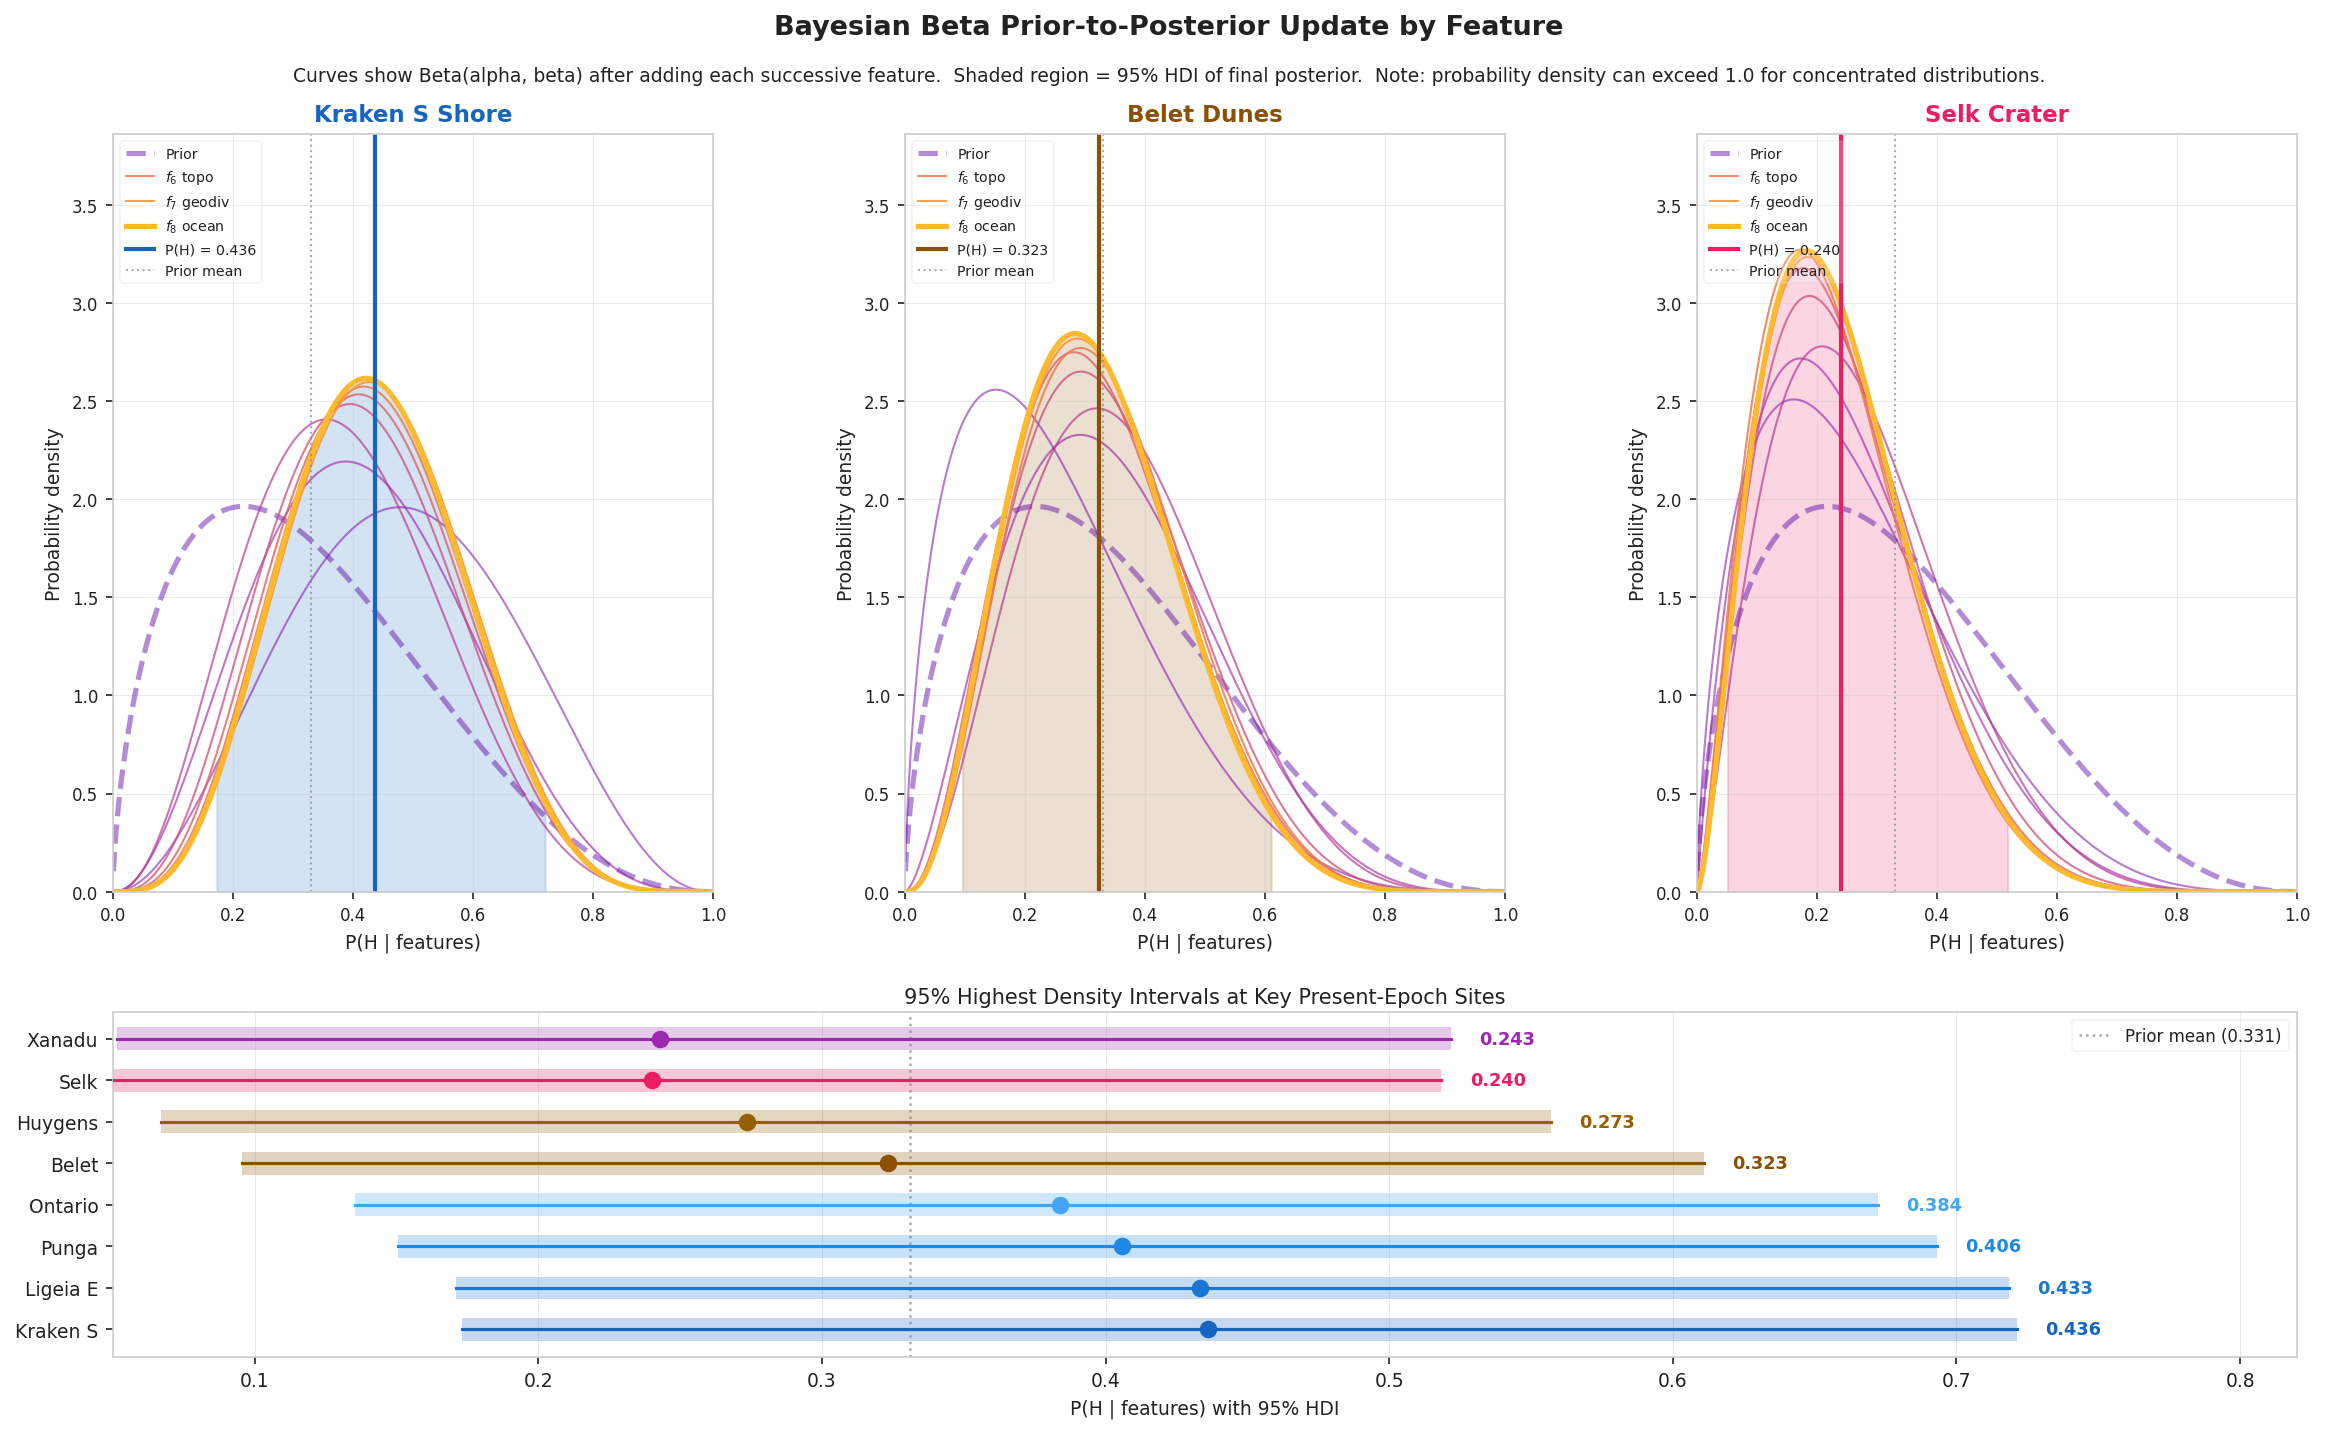
\includegraphics[width=\textwidth]{images/beta_update_figure.png}
  \caption{Beta prior-to-posterior update for three representative sites.
    \textit{Top row:} each curve shows the Beta distribution
    $\mathrm{Beta}(\alpha_0 + \lambda\sum w_if_i,\;
    \beta_0 + \lambda\sum w_i(1-f_i))$ after incorporating successive
    features, from the prior (dashed) through to the 8-feature posterior
    (solid).  Shaded region = 95\% HDI of the final posterior.
    The vertical dotted line marks the prior mean $\mu_0 = 0.331$.
    \textit{Bottom panel:} 95\% HDI bars for eight key present-epoch
    sites, sorted by posterior mean.  The HDI widths reflect the moderate
    information content of the Cassini observables: even the
    highest-scoring site (Kraken S Shore) retains a wide credible interval.
    Generated by \texttt{scripts/generate\_beta\_update\_figure.py};
    output at \texttt{outputs/diagnostics/beta\_update\_figure.pdf}.}
  \label{fig:beta_update}
\end{figure}

\subsection{Missing Data Imputation}
\label{sec:nan}

Where a feature is absent at a pixel (data coverage gap), it is imputed
with its prior mean $\mu_i$ before the update.  Substituting $f_i = \mu_i$
into Equations~\ref{eq:alpha_post}--\ref{eq:beta_post} adds $\lambda w_i \mu_i$
to $\alpha_\text{post}$ and $\lambda w_i(1 - \mu_i)$ to $\beta_\text{post}$
--- exactly the amounts the prior already encodes for that feature.  The net
effect is zero: a missing observation contributes no evidence.  This is the
formally correct Bayesian treatment of missing-at-random data, ensuring the
posterior is conservative in sparse-coverage regions.

\subsection{Feature Importance Validation}
\label{sec:classifier}

The Bayesian posterior map (Eq.~\ref{eq:posterior_mean}) is the primary
scientific result.  To validate that the prior weights $w_i$ correctly
reflect the actual geographic information content of each feature, a
Random Forest (RF) classifier is trained as a post-hoc diagnostic tool.

Binary labels are derived from the Bayesian posterior map by 50/50 median
split: pixels above the global spatial median receive a positive
\lq\lq habitable\rq\rq{} label.  A Random Forest classifier
\citep{Breiman2001} is trained on these labels and isotonically calibrated.
Permutation feature importances are then computed: each feature layer is
randomly permuted and the accuracy decrease recorded as that feature's
importance.  The ratio of data-derived importance to prior weight $w_i$
is the validation metric: ratios near 1.0 for all features confirm that
the prior weight specification is consistent with the observed spatial
discrimination (Section~\ref{sec:importances}).

\textit{Note:} The RF classifier outputs are not used as scientific
results.  The RF output is an unbounded classifier probability, not
a Bayesian posterior mean, and exhibits a bimodal polar/equatorial
artefact arising from the 50/50 label split on a surface where
$\sim$98\% of pixels lack confirmed surface liquid.  All $P(H)$
values reported in Chapter~\ref{ch:results} are from
Eq.~\ref{eq:posterior_mean} directly.

\section{Temporal Configurations}
\label{sec:temporal_configs}

\subsection{Design Philosophy}
\label{sec:temporal_design}

The habitability framework is applied at five distinct temporal configurations,
each representing a qualitatively different physical state of \titan{}.  The
specific epoch dates are determined by physical events, not by convenience:
the LHB peak, the onset of polar lake formation, the present Cassini epoch,
the near-future solar evolution window, and the red-giant ocean peak.  At
each anchor epoch, the eight features are given physically motivated prior
means and epoch-specific feature configurations that modify which features
are active and how they should be interpreted.

\subsection{\textit{Past} Epoch: Late Heavy Bombardment ($\sim\!\!-3.5$\,Gya)}
\label{sec:epoch_past}

The LHB ($\sim$$-4.1$ to $-3.8\gya$; \citealt{Gomes2005}) produced water--ammonia--organic melt ponds persisting $10^3$--$10^4$\,yr at confirmed crater sites \citep{OBrien2005}.  No stable polar hydrocarbon seas existed.  Impact-melt proximity and cryovolcanic flux features are active; liquid hydrocarbon is proxied by melt-pond coverage ($\mu_1=0.025$); organic accumulation is at $\sim$40\% of present-day levels ($\mu_2=0.30$); methane cycle is episodic ($\mu_4=0.20$); subsurface ocean proximity is 2.5$\times$ elevated ($s_8=2.5$) reflecting the thinner ice shell.

\subsection{\textit{Lake Formation} Epoch ($\sim\!\!-1.0$\,Gya)}
\label{sec:epoch_lf}

Polar lakes are consolidating: $f_1$ ramps from 10\% to 100\% of present between $-1.0$ and $-0.5\gya$.  Organic accumulation reaches $\sim$75\% of the present level; the methane rain cycle is becoming established.

\subsection{\textit{Present} Epoch: Cassini Era (2004--2017)}
\label{sec:epoch_present}

All features at present-epoch values.  Feature maps are the Cassini observational layers described in Section~\ref{sec:data}.  This epoch is the sole anchor for which direct observational posteriors are available.

\subsection{\textit{Near Future} Epoch ($+0.25$\,Gya)}
\label{sec:epoch_nf}

Solar luminosity is $\sim$1.4\% above present \citep{Bahcall2001}; all features unchanged within model resolution.  The ranking is analytically identical to the \textit{Present} epoch.

\subsection{\textit{Future} Epoch: Red-Giant Ocean Peak ($+5.9$\,Gya)}
\label{sec:epoch_future}

At $+5.1\gya$ surface temperature crosses the water--ammonia eutectic (176\,K; \citealt{Grasset2005}).  Liquid hydrocarbon gives way to a global water--ammonia ocean ($f_1 \to 1.0$ everywhere); subsurface ocean merges with the surface ocean ($f_8 \to 1.0$); organic accumulation reaches $2.5\times$ the present-epoch level.  The methane cycle becomes a water cycle; acetylene photochemistry is suppressed under the water-ammonia atmosphere \citep{Lorenz1997}.

\section{Multi-Epoch Habitability Reconstruction}
\label{sec:multi_epoch}

\subsection{Temporal Scaling of Features}
\label{sec:epoch_scaling}

The multi-epoch reconstruction applies epoch-specific scale functions to the present-epoch feature maps:
\begin{equation}
  f_i(t) = \text{clip}\bigl[\,s_i(t)\cdot f_i(0),\;0,\;1\bigr]
  \label{eq:temporal_scale}
\end{equation}
where $s_i(t)$ is the scale multiplier for feature $i$ at epoch $t$ (Table~\ref{tab:scale_funcs}).  Two time constants appear in the scale functions: $t_\odot = 4.57\gya$, the current age of the Sun \citep{Bahcall2001}, which governs UV-dependent features ($s_3$, $s_1$ at red-giant epochs); and $t_\text{atm} = 4.0\,\text{Gyr}$, the estimated duration of active tholin photochemistry in \titan{}'s atmosphere, which governs organic accumulation ($s_2$).  The posterior is evaluated at each pixel using the scaled features and 72 epochs spanning $-3.8\gya$ to $+6.5\gya$.  An epoch-aware PCHIP interpolation between anchor posteriors provides smooth transitions between static-pipeline anchor states.


\begin{table}[H]
\centering
\small
\caption{Temporal scale functions $s_i(t)$ applied to each feature at epoch $t$
  (Gyr from present), with supporting references.  A multiplier of 1.0 means
  no change from the present-epoch value; values $< 1$ reduce the feature,
  values $> 1$ enhance it.  All outputs are clipped to $[0, 1]$ after scaling.
  The eutectic override ($T_s \geq 176\,\mathrm{K}$) applies to $f_1$, $f_3$,
  $f_4$, and $f_8$ at the red-giant ocean epoch
  \citep{Grasset2005,Tobie2005,Lorenz1997}.}
\label{tab:scale_funcs}
\begin{tabular}{p{2.2cm}p{7.0cm}p{3.6cm}}
\toprule
\textbf{Feature} & \textbf{Scale function $s_i(t)$} & \textbf{Key references} \\
\midrule
$f_1$ liquid HC &
  0.10 for $t < -1.0\gya$ (pre-lake era); ramps $0.1\to1.0$ from $-1.0$ to
  $-0.5\gya$ (lake establishment); 1.0 until $+4.0\gya$; declines linearly
  to 0 by $+5.0\gya$ (solar evaporation);
  overridden to 1.0 (global ocean) at $T_s \geq 176\,\mathrm{K}$. &
  \citet{Tobie2006,MitchellLora2016,Lorenz1997,Hayes2016} \\[4pt]

$f_2$ organic &
  $\min\!\bigl((t_\text{atm}\!+\!t)/t_\text{atm},\;2.5\bigr)$: linear accumulation of
  UV-photolysed tholins proportional to atmospheric age since $\sim$$-4.0\gya$;
  capped at $2.5\times$ present.  \emph{Declared approximation}: a constant
  production rate is assumed; the actual rate was higher under the younger,
  more UV-active Sun (see $s_3$). &
  \citet{Lavvas2011,Cable2012,Vuitton2007,Niemann2005} \\[4pt]

$f_3$ acetylene &
  $(t_\odot/(t_\odot\!+\!t))^{0.5}$: UV-driven C$_2$H$_2$ production scales with
  solar EUV/FUV luminosity; young Sun was more active.  Overridden to
  $0.10/0.35$ under global ocean (UV shielded). &
  \citet{Strobel2010,Lavvas2011,Bahcall2001,Loison2015} \\[4pt]

$f_4$ methane &
  0.60 for $t < -1.0\gya$ (episodic outgassing, pre-lake); 0.80 for
  $-1.0$ to $-0.5\gya$; 1.0 until $+4.5\gya$; declines to 0 by $+5.0\gya$
  (Jeans escape and photolytic loss).  Overridden to $0.30/0.40$ under
  global ocean. &
  \citet{Tobie2006,Niemann2005,Flasar2005,MitchellLora2016,Strobel2010} \\[4pt]

$f_5$ surf--atm &
  $0.40 + 0.60\,s_1(t)$: fixed slope-transport component (0.40) reflects
  aeolian and hillslope processes independent of liquid presence; lake-margin
  evaporation--condensation exchange (0.60) scales directly with liquid
  coverage $s_1(t)$. &
  \citet{Radebaugh2011,Hayes2016,MitchellLora2016} \\[4pt]

$f_6$ topo &
  1.30 for $t < -2.0\gya$; 1.15 for $-2.0$ to $-1.0\gya$; 1.0 thereafter.
  Higher roughness at early epochs reflects greater impact crater density;
  craters are progressively buried and eroded on timescales of $\sim$1--2\,Gyr. &
  \citet{Lorenz2013,Artemieva2003,Hedgepeth2020,Neish2010} \\[4pt]

$f_7$ geodiv &
  0.70 for $t < -3.0\gya$; 0.85 for $-3.0$ to $-2.0\gya$; 1.0 thereafter.
  Early terrain dominated by impact ejecta (low class diversity); lacustrine
  plains, dune fields, and shorelines accumulate to yield present-day eight-class
  diversity \citep{Lopes2019}. &
  \citet{Lopes2019,Artemieva2003,Malaska2020,Hayes2016} \\[4pt]

$f_8$ ocean &
  2.50 for $t < -2.0\gya$; 1.80 for $-2.0$ to $-1.0\gya$;
  1.30 for $-1.0$ to $-0.5\gya$; 1.0 thereafter.
  Thicker ice shell at earlier epochs places the subsurface ocean closer
  to the surface; shell thickens as radiogenic heat declines.
  Overridden to $1.0/0.03$ at $T_s \geq 176\,\mathrm{K}$ (ocean is
  at the surface). &
  \citet{Iess2012,Tobie2005,Nimmo2010,Mitri2014,Grasset2005} \\
\bottomrule
\end{tabular}
\end{table}


\paragraph{Animation model weights.}  The animation model includes a ninth
synthesised feature, \texttt{impact\_melt\_bonus} ($w = 0.09$,
$\mu = 0.00$), which adds a spatially uniform LHB-era melt-pond signal at
past epochs and is zero everywhere at the present epoch
\citep{Artemieva2003,Neish2009,Neish2018}.  The bonus follows a Gaussian
centred on $-3.8\gya$ (Late Heavy Bombardment peak; \citealt{Gomes2005}) with a
half-width of 500\,Myr, consistent with the crater flux decay timescale.
To accommodate this ninth feature while keeping $\sum w_i = 1.0$, all eight
standard feature weights are reduced by $\approx 0.02$ relative to the pipeline
values in Table~\ref{tab:priors}.  Consequently the animation
$\mu_0 = 0.299$ differs from the pipeline value of $0.331$; the
\texttt{\_rescale\_bayesian()} linear mapping corrects this before display.

The key scale functions encode the following physical transitions:
\begin{itemize}
  \item \textbf{Liquid hydrocarbon} ($s_1$): held at 0.10 (10\% of
    present) for $t < -1.0\gya$, reflecting the episodic methane outgassing
    model of \citet{Tobie2006} in which sustained lake coverage is a
    geologically recent development.  The ramp from $-1.0$ to $-0.5\gya$
    corresponds to consolidation of Kraken Mare and Ligeia Mare
    \citep{Hayes2016,MitchellLora2016}.  Decline to zero by $+5.0\gya$ is
    driven by increasing solar luminosity vaporising the seas
    \citep{Lorenz1997}.  The water--ammonia eutectic temperature of
    176\,K \citep{Grasset2005,Tobie2005} triggers the global-ocean override.

  \item \textbf{Organic abundance} ($s_2$): the linear form
    $\min(t_{\rm elapsed}/4\,\mathrm{Gyr},\,2.5)$ approximates
    steady-state UV photolysis of CH$_4$ accumulating tholins since
    \titan{}'s atmosphere formed $\sim 4\gya$ \citep{Niemann2005,Tobie2006}.
    Tholin synthesis rates under Cassini-era conditions are quantified in
    \citet{Lavvas2011} and \citet{Cable2012}.  The declared approximation
    of a constant production rate underestimates early-epoch organic
    accumulation, since UV flux was higher under the younger Sun (see $s_3$).

  \item \textbf{Chemical energy} ($s_3$): the $(L_\odot(t)/L_\odot)^{0.5}$
    scaling follows the solar standard luminosity evolution of
    \citet{Bahcall2001}, applied to UV-driven acetylene production
    \citep{Strobel2010,Loison2015}.  A younger, more UV-active Sun produced
    proportionally more C$_2$H$_2$ \citep{Lavvas2011}.  The $^{0.5}$ exponent
    is a conservative estimate; EUV scaling is steeper \citep{Sagan1979}.

  \item \textbf{Methane cycle} ($s_4$): the step at $-1.0\gya$ (0.60 to 0.80)
    and ramp to 1.0 at $-0.5\gya$ encode the \citet{Tobie2006} three-episode
    cryovolcanic outgassing model, in which sustained methane cycling
    post-dates lake formation \citep{Flasar2005,Niemann2005}.  Future
    depletion follows escape flux estimates of \citet{Strobel2010}.

  \item \textbf{Topographic complexity} ($s_6$): the elevated values
    at $t < -2.0\gya$ reflect higher impact crater density at early epochs
    \citep{Artemieva2003}.  Crater obliteration timescales of 1--2\,Gyr,
    inferred from the observed low crater density \citep{Hedgepeth2020}
    and crater degradation studies \citep{Neish2010}, motivate the step
    function transitions.

  \item \textbf{Geomorphologic diversity} ($s_7$): the monotone increase
    towards the present reflects the progressive accumulation of distinct
    terrain classes in the \citet{Lopes2019} geomorphological map.
    Early terrain is impact-dominated \citep{Artemieva2003}; lacustrine
    and aeolian classes accrue from $\sim -1.0\gya$ \citep{Malaska2020}.

  \item \textbf{Subsurface ocean} ($s_8$): the 2.5$\times$ enhancement at
    $t < -2.0\gya$ is calibrated to the thermal evolution model of
    \citet{Tobie2005}, in which a thinner ice shell at early epochs places
    the subsurface ocean closer to potential surface-chemistry pathways.
    Shell-thickening as radiogenic heating declines is modelled by
    \citet{Nimmo2010} and \citet{Mitri2014}; the present-day ocean depth
    is confirmed by \citet{Iess2012}.
\end{itemize}

\subsection{Validation}
\label{sec:validation}

The reconstruction is validated by checking that: (i)~each anchor epoch's scaled posterior is within 0.02 of the corresponding static-pipeline posterior at the 95th percentile; (ii)~the global mean rises monotonically through the lake-formation transition; and (iii)~the N-polar/equatorial ratio follows the expected pattern (unity at LHB; $>$2 at present; falling to unity at the global ocean).  All three criteria are satisfied.

\section{Scope of This Thesis}
\label{sec:scope_methods}

The primary analysis presented in Chapters~\ref{ch:results} and
\ref{ch:discussion} focuses on the five static epoch habitability maps and
the temporal evolution described through the multi-epoch reconstruction.
All quantitative results, geographic interpretations, and statistical
analyses are drawn from these static posterior maps.  The implementation
is carried out in Python 3.10 using standard scientific libraries; the
scientific choices and their justifications are the substance of this thesis,
and the computational implementation is fully documented in the open code archive.
